\documentclass[tikz,border=8pt]{standalone}
\usepackage{amsmath,amssymb}
\usepackage{tikz}
% Lightweight Feynman slash without external packages
\providecommand{\slashed}[1]{\ensuremath{\not\!#1}}
\usetikzlibrary{arrows.meta,calc,decorations.pathreplacing,patterns,shapes.geometric,positioning,shadings,decorations.markings,decorations.pathmorphing}

\begin{document}
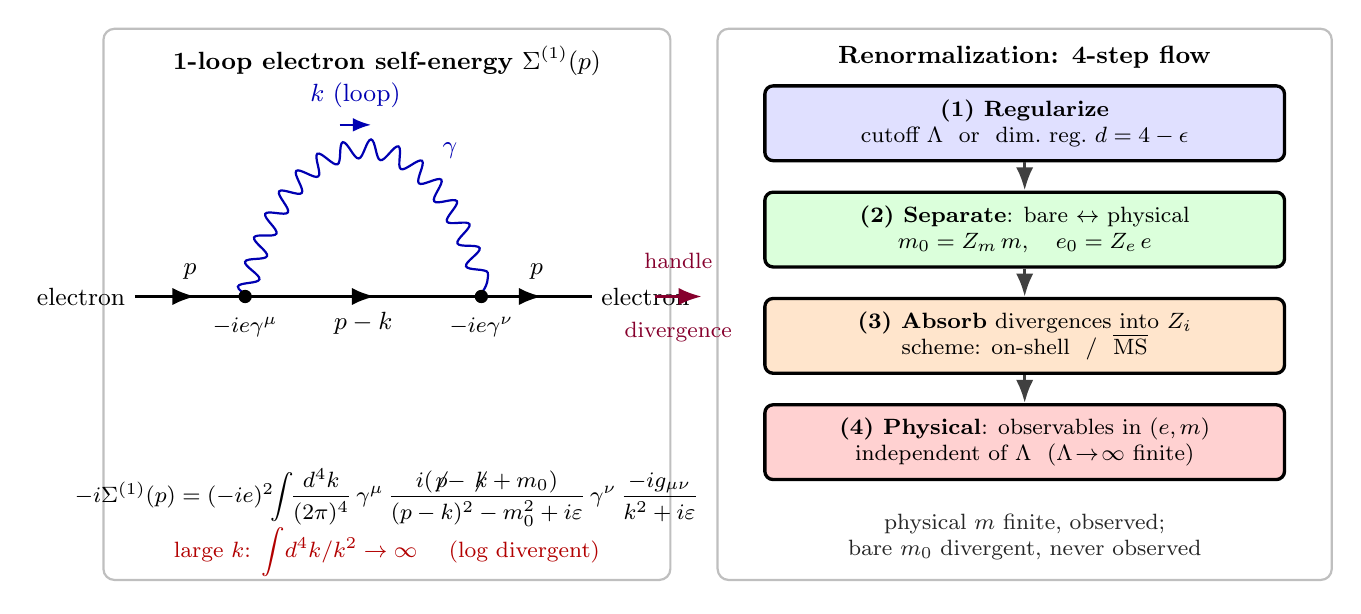
\begin{tikzpicture}[>=Latex, font=\small]

% =========================================================
% LEFT PANEL: One-loop electron self-energy Feynman diagram
% =========================================================

% Frame for left panel
\draw[rounded corners=4pt, thick, gray!50]
  (-7.4,-3.6) rectangle (-0.2,3.4);
\node[anchor=north] at (-3.8,3.3)
  {\textbf{1-loop electron self-energy} $\Sigma^{(1)}(p)$};

% Coordinates for the diagram
% Incoming electron at left, vertex A; outgoing electron at right, vertex B
\coordinate (Pin)  at (-7.0, 0.0);
\coordinate (A)    at (-5.6, 0.0);
\coordinate (B)    at (-2.6, 0.0);
\coordinate (Pout) at (-1.2, 0.0);

% Incoming electron line with arrow (momentum p)
\draw[very thick, black, postaction={decorate,
  decoration={markings, mark=at position 0.55 with {\arrow{Latex}}}}]
  (Pin) -- (A);
\node[above] at ($(Pin)!0.5!(A) + (0,0.1)$) {$p$};

% Outgoing electron line with arrow (momentum p)
\draw[very thick, black, postaction={decorate,
  decoration={markings, mark=at position 0.55 with {\arrow{Latex}}}}]
  (B) -- (Pout);
\node[above] at ($(B)!0.5!(Pout) + (0,0.1)$) {$p$};

% Internal electron line between vertices A and B (momentum p-k)
\draw[very thick, black, postaction={decorate,
  decoration={markings, mark=at position 0.55 with {\arrow{Latex}}}}]
  (A) -- (B);
\node[below=2pt] at ($(A)!0.5!(B)$) {$p-k$};

% Photon loop arc above (wavy line) connecting A to B
% The photon carries loop momentum k
\draw[thick, blue!70!black,
      decorate, decoration={snake, amplitude=1.2mm, segment length=3.2mm}]
  (A) .. controls (-5.0,2.4) and (-3.2,2.4) .. (B);

% Arrow indicating photon loop momentum k
\draw[->, thick, blue!70!black]
  (-4.4, 2.18) -- (-4.0, 2.18);
\node[blue!70!black] at (-4.2, 2.55) {$k$ (loop)};

% Photon label
\node[blue!70!black] at (-3.0, 1.85) {$\gamma$};

% Vertices (filled dots)
\filldraw[black] (A) circle (2.2pt);
\filldraw[black] (B) circle (2.2pt);

% Vertex coupling labels
\node[below=4pt, font=\footnotesize] at (A) {$-ie\gamma^{\mu}$};
\node[below=4pt, font=\footnotesize] at (B) {$-ie\gamma^{\nu}$};

% Endpoint labels
\node[left]  at (Pin)  {electron};
\node[right] at (Pout) {electron};

% Caption beneath the diagram
\node[align=center, font=\footnotesize] at (-3.8,-2.55)
  {$-i\Sigma^{(1)}(p)=(-ie)^{2}\!\!\displaystyle\int\!\!\frac{d^{4}k}{(2\pi)^{4}}\,
   \gamma^{\mu}\,\dfrac{i(\slashed{p}-\slashed{k}+m_{0})}{(p-k)^{2}-m_{0}^{2}+i\varepsilon}\,
   \gamma^{\nu}\,\dfrac{-ig_{\mu\nu}}{k^{2}+i\varepsilon}$};

\node[align=center, font=\footnotesize, red!70!black] at (-3.8,-3.25)
  {large $k$: $\displaystyle\int\!d^{4}k/k^{2}\to\infty$ \quad (log divergent)};

% =========================================================
% RIGHT PANEL: Renormalization 4-step flow chart
% =========================================================

% Frame for right panel
\draw[rounded corners=4pt, thick, gray!50]
  (0.4,-3.6) rectangle (8.2,3.4);
\node[anchor=north] at (4.3,3.3)
  {\textbf{Renormalization: 4-step flow}};

% Step boxes (vertical column)
\tikzset{
  stepbox/.style={
    rounded corners=3pt,
    draw=black, very thick,
    fill=#1,
    minimum width=6.6cm,
    minimum height=0.95cm,
    align=center,
    font=\footnotesize
  },
  stepbox/.default=yellow!15
}

% Step 1: Regularize
\node[stepbox=blue!12]   (S1) at (4.3, 2.20)
  {\textbf{(1) Regularize} \\
   cutoff $\Lambda$ \ or \ dim.\ reg.\ $d=4-\epsilon$};

% Step 2: Separate
\node[stepbox=green!14]  (S2) at (4.3, 0.85)
  {\textbf{(2) Separate}: bare $\leftrightarrow$ physical \\
   $m_{0}=Z_{m}\,m, \quad e_{0}=Z_{e}\,e$};

% Step 3: Absorb
\node[stepbox=orange!20] (S3) at (4.3,-0.50)
  {\textbf{(3) Absorb} divergences into $Z_{i}$ \\
   scheme: on-shell \ / \ $\overline{\mathrm{MS}}$};

% Step 4: Physical
\node[stepbox=red!18]    (S4) at (4.3,-1.85)
  {\textbf{(4) Physical}: observables in $(e,m)$ \\
   independent of $\Lambda$ \ ($\Lambda\!\to\!\infty$ finite)};

% Arrows between steps
\draw[->, very thick, black!75] (S1.south) -- (S2.north);
\draw[->, very thick, black!75] (S2.south) -- (S3.north);
\draw[->, very thick, black!75] (S3.south) -- (S4.north);

% Bottom annotation
\node[align=center, font=\footnotesize, gray!30!black]
  at (4.3,-3.05)
  {physical $m$ finite, observed; \\
   bare $m_{0}$ divergent, never observed};

% =========================================================
% Connector arrow from left diagram to flow chart
% =========================================================
\draw[->, very thick, purple!70!black]
  (-0.4, 0.0) -- (0.2, 0.0);
\node[purple!70!black, font=\footnotesize, align=center]
  at (-0.1, 0.45) {handle};
\node[purple!70!black, font=\footnotesize, align=center]
  at (-0.1,-0.45) {divergence};

\end{tikzpicture}
\end{document}
